\section{Integral Formulas}
\label{sec:formulas}
% From Section 3.3
Now we can put the ideas of areas and antiderivatives together to get a way of evaluating definite integrals that is exact and often easy. To evaluate a definite integral $\displaystyle\int_a^b f(t)\,dt$, we can find any antiderivative $F(t)$ of $f(t)$ and evaluate $F(b)-F(a)$. The problem of finding the exact value of a definite integral reduces to finding some (any) antiderivative $f(x)$ of the integrand and then evaluating $F(b)-F(a)$. Even finding one antiderivative can be difficult, and we will stick to functions that have easy antiderivatives.

\subsection{Building Blocks}
Antidifferentiation is going backwards through the derivative process. So the easiest antiderivative rules are simply backwards versions of the easiest derivative rules. Recall the following from Chapter \ref{ch:derivatives}.

\begin{theorem}[Derivative Rules: Building Blocks]
In what follows, $f(x)$ and $g(x)$ are differentiable functions of $x$.

\noindent{\bf Constant Multiple Rule}
$$\dfrac{d}{\, dx }kf=kf'$$
{\bf Sum and Difference Rule}
$$\dfrac{d}{\, dx }(f\pm g)=f'\pm g'$$
{\bf Power Rule}
$$\dfrac{d}{\, dx }x^n=nx^{n-1}$$
{\bf Special cases:}
$$\dfrac{d}{\, dx }k = 0 \quad (\text{Because }k=kx^0.)$$
$$\dfrac{d}{\, dx }x = 1 \quad (\text{Because }x=x^1.)$$
{\bf Exponential Functions}
$$\dfrac{d}{\, dx }e^x=e^x$$
$$\dfrac{d}{\, dx }a^x=\ln(a)a^x$$
{\bf Natural Logarithm}
$$\dfrac{d}{\, dx }\ln(x)=\dfrac{1}{x}$$
\end{theorem}
Thinking about these basic rules was how we came up with the antiderivatives of $2x$ and $e^x$ before.

The corresponding rules for antiderivatives are next – each of the antiderivative rules is simply rewriting the derivative rule. All of these antiderivatives can be verified by differentiating.

There is one surprise – the antiderivative of $\dfrac{1}{x}$ is actually not simply $\ln(x)$, it's $\ln(|x|)$. This is a good thing – the antiderivative has a domain that matches the domain of $\dfrac{1}{x}$, which is bigger than the domain of $\ln(x)$, so we don’t have to worry about whether our $x$'s are positive or negative. But we must be careful to include those absolute values – otherwise, we could end up with domain problems.

\begin{theorem}[Antiderivative Rules: Building Blocks]
In what follows, $f(x)$ and $g(x)$ are differentiable functions of $x$, and $k$, $n$, and $C$ are constants.

\noindent{\bf Constant Multiple Rule}
$$\int k\cdot f(x)\, dx = k\cdot \int f(x)\, dx $$
{\bf Sum and Difference Rule}
$$\int(f(x)\pm g(x))\, dx = \int f(x)\, dx \pm \int g(x)\, dx $$
{\bf Power Rule}
$$\int x^n\, dx = \frac{x^{n+1}}{n+1} + C, \quad\text{provided that }n\neq -1$$
{\bf Special case:}
$$\int k\, dx = kx+C \quad (\text{Because }k=kx^0.)$$
(The other special case ($n=-1$) is covered next.)

\noindent{\bf Natural Logarithm}
$$\int x^{-1}\, dx = \int \frac{1}{x}\, dx = \ln(|x|)+C$$
{\bf Exponential Functions}
$$\int e^x\, dx = e^x+C$$
$$\int a^x\, dx = \frac{a^x}{\ln(a)} + C$$
\end{theorem}

\begin{example}
Find the antiderivative of $y=3x^7-15\sqrt{x} + \dfrac{14}{x^2}$.

\begin{solution}
\begin{align*}
\int\left(3x^7-15\sqrt{x} + \dfrac{14}{x^2}\right)\, dx &= \int\left(3x^7-15x^{1/2} + 14x^{-2}\right)\, dx \\
  &=  3\frac{x^8}{8} - 15 \frac{x^{3/2}}{3/2} + 14\frac{x^{-1}}{-1} + C\\
  &= \frac{3}{8}x^8 - 10x^{3/2} - 14x^{-1} + C
\end{align*}
\end{solution}\end{example}

\begin{example}
Find $\displaystyle\int\left(e^x+12-\frac{16}{x}\right)\, dx$.

\begin{solution}
  $$\int\left(e^x+12-\frac{16}{x}\right)\, dx =e^x+12x-16\ln(|x|)+C$$
\end{solution}\end{example}

\begin{example}
Find $F(x)$ so that $F'(x)=e^x$ and $F(0)=10$.

\begin{solution}
This time we are looking for a particular antiderivative; we need to find exactly the right constant. Let's start by finding the antiderivative:
$$\int e^x\, dx = e^x+C \enspace .$$
So we know that $F(x)=e^x+C$, for some real number $C$. Now we just need to find which one. To do that, we'll use the other piece of information (the initial condition):
\begin{align*}
F(x) &= e^x+C \\
F(0) &= e^0+C = 1+C=10 \\
C &= 9
\end{align*}
The particular constant we need is 9; thus, $F(x) = e^x + 9$.
\end{solution}\end{example}

The reason we are looking at antiderivatives right now is so we can evaluate definite integrals exactly. Recall the Fundamental Theorem of Calculus:

$$\int_a^b F'(x)\, dx =F(b)-F(a) \enspace .$$
If we can find an antiderivative for the integrand, we can use that to evaluate the definite integral. The evaluation $F(b)-F(a)$ is represented as $\left. F(x)\right|_a^b$.

\begin{example}
  \label{ex:5-5-line}
Evaluate $\displaystyle\int_1^3 x\, dx$  in two ways.
  \begin{enumerate}[label=(\alph*)]
    \item By sketching the graph of $y=x$ and geometrically finding the area.

    \begin{solution}
      The graph of $y=x$ is shown in Figure \ref{fig:5-5-line}, and the shaded region corresponding to the integral has area 4.

      \begin{figure}[!ht]
        \centering
          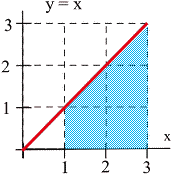
\includegraphics[width=0.3\textwidth]{img/chap5/image043.png}
          \caption{Graph for Example \ref{ex:5-5-line}.}
          \label{fig:5-5-line}
      \end{figure}
    \end{solution}
    \item By finding an antiderivative of $F(x)$ of the integrand and evaluating $F(3)-F(1)$.

      \begin{solution}
        One antiderivative of $x$ is $F(x)=\frac{1}{2}x^2$, and
         \begin{align*}
         \int_1^3 x\, dx &= \left.\frac{1}{2}x^2\right|_1^3 \\
         &= \left(\frac{1}{2}(3)^2\right) - \left(\frac{1}{2}(1)^2\right)\\
         &= \frac{9}{2} - \frac{1}{2} \\
         &= 4.
       \end{align*}
     Note that this answer agrees with the answer we got geometrically.

     If we had used another antiderivative of $x$, say $F(x)=\frac{1}{2}x^2+7$, then
     \begin{align*}
     \int_1^3 x\, dx &= \left.\frac{1}{2}x^2 + 7\right|_1^3 \\
     &= \left(\frac{1}{2}(3)^2+ 7\right) - \left(\frac{1}{2}(1)^2+ 7\right)\\
     &= \frac{9}{2}+ 7 - \frac{1}{2} - 7 \\
     &= 4.
     \end{align*}
     In general, whatever constant we choose gets subtracted away during the evaluation, so we might as well always choose the easiest one, where the constant is 0.
     \end{solution}
   \end{enumerate}
\end{example}

\begin{example}
Find the area between the graph of $y=3x^2$ and the horizontal axis for $x$ between 1 and 2.

\begin{solution}
  This is
  $$\int_1^2 3x^2\, dx = \left. x^3 \right|_1^2 = 2^3-1^3=7 \enspace .$$
\end{solution}\end{example}

\begin{example}
A robot has been programmed so that when it starts to move, its velocity after $t$ seconds will be $3t^2$ feet/second.
  \begin{enumerate}[label=(\alph*)]
    \item How far will the robot travel during its first 4 seconds of movement?

    \begin{solution}
      The distance during the first 4 seconds will be the area under the graph of velocity, from $t=0$ to $t=4$.

      \begin{figure}[!ht]
        \centering
          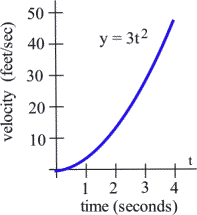
\includegraphics[width=0.3\textwidth]{img/chap5/image044.png}
          \caption{Robot velocity after $t$ seconds}
          \label{fig:5-5-robot}
      \end{figure}
That area is the definite integral $\displaystyle\int_0^4 3t^2\,dt$. An antiderivative of $3t^2$ is $t^3$, so $\displaystyle\int_0^4 3t^2\,dt = \left.t^3\right|_0^4 = 4^3-0^3=64$ feet.
      \end{solution}
    \item How far will the robot travel during its next 4 seconds of movement?

    \begin{solution}
      $\displaystyle\int_4^8 3t^2\, dt = \left.t^3\right|_4^8 = 8^3-4^3=512-64=448$ feet.
      \end{solution}
  \end{enumerate}
\end{example}

\begin{example}
Suppose that $t$ minutes after putting 1000 bacteria on a Petri plate the rate of growth of the population is $6t$ bacteria per minute.
  \begin{enumerate}[label = (\alph*)]
    \item How many new bacteria are added to the population during the first 7 minutes?

    \begin{solution}
      The number of new bacteria is the area under the rate of growth graph in Figure \ref{fig:5-5-bacteria}, and one antiderivative of $6t$ is $3t^2$.

      \begin{figure}[!ht]
        \centering
          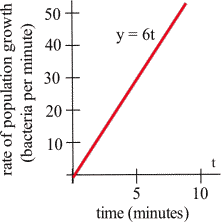
\includegraphics[width=0.3\textwidth]{img/chap5/image045.png}
          \caption{Bacteria growth rate after $t$ minutes.}
          \label{fig:5-5-bacteria}
      \end{figure}
      So the number of new bacteria is
      $$\int_0^7 6t\,dt = \left. 3t^2 \right|_0^7 = 3(7)^2-3(0)^2 = 147 \enspace .$$
      \end{solution}
    \item What is the total population after 7 minutes?

    \begin{solution}
      Therefore, the new population is the old population plus the new bacteria: $1000 + 147 = 1147$ bacteria.
      \end{solution}
  \end{enumerate}
\end{example}

\begin{example}
A company determines their marginal cost for production, in dollars per item, is $MC(x)=\dfrac{4}{\sqrt{x}}+2$ when producing $x$ thousand items. Find the cost of increasing production from 4 thousand items to 5 thousand items.

\begin{solution}
  Remember that marginal cost is the rate of change of cost, and so the fundamental theorem tells us that
  $$\int_a^b MC(x)\, dx = \int_a^b C'(x)\, dx =C(b)-C(a) \enspace .$$
  In other words, the integral of marginal cost will give us a net change in cost. To find the cost of increasing production from 4 thousand items to 5 thousand items, we need to integrate $\displaystyle\int_4^5 MC(x)\, dx$.

We can write the marginal cost as $MC(x)=4x^{-1/2}+2$. We can then use the basic rules to find an antiderivative:
$$C(x) = 4\frac{x^{1/2}}{1/2} + 2x = 8\sqrt{x} + 2x\enspace .$$
Using this, the net change in cost is
\begin{align*}
  \int_4^5\left(4x^{-1/2}+2\right)\, dx &= \left.\left(8\sqrt{x} + 2x\right)\right|_4^5 \\
  &= (8\sqrt{5} - 2(5)) - (8\sqrt{4} +2(4))\\
  &\approx 3.889
\end{align*}
It will cost about 3.889 thousand dollars to increase production from 4 thousand items to 5 thousand items. (The final answer would be better written as \$3889.)
\end{solution}\end{example}
